\newpage
\section{Backtracking}

\subsection{Introduccion}

El backtracking es una técnica de diseño de algoritmos para resolver problemas 
combinatorios.
Consiste en construir soluciones parciales y retroceder cuando se determina que 
una solución parcial no puede llevar a una solución completa válida.

\subsection{Fuerza Bruta (Brute Force)}

La fuerza bruta busca en todo el espacio de soluciones posibles para encontrar
las validas y elegir la mejor entre ellas. Es una tecnica simple pero costosa, asi 
que es mejor utilizarla cuando el espacio de soluciones sea pequeno.

\begin{multicols}{2}
\setlength{\parindent}{0pt}
\subsubsection*{Permutaciones}

Forma de ordenar los elementos de un conjunto de forma
específica.

\begin{center}
    $[1,2,3], [1,3,2], [2,1,3], [2,3,1], [3,1,2], [3,2,1]$
\end{center}

En C++ se puede usar la función \textbf{next\_permutation} para generar todas las 
permutaciones de un conjunto.\\

\begin{lstlisting}
/*Generar todas las permutaciones de conjunto*/
vector<int> conjunto = {1,2,3,4};
do {
    // Imprime la permutacion actual 
    for (auto numero : conjunto)
        cout << c << " ";
        cout << endl;
} while(next_permutation(conjunto.begin(),conjunto.end()));
// Tiempo: O(n!)
// Espacio: O(1)
\end{lstlisting}

\newcolumn
\subsubsection*{Subconjuntos}

Serie de elementos que pertenecen a un conjunto original, pero no necesariamente 
conserva todos los elemento.\\

\begin{center}
    $\{\varnothing\}, \{1\}, \{2\}, \{1,2\}, \{3\}, \{1,3\}, \{2,3\}, \{1,2,3\}$
\end{center}

Una tecnica para generar subconjuntos es usar ''masking''. Cada bit representa si un
elemento pertenece o no al subconjunto.

\begin{center}
    \begin{tabular}{|c|c|c|c|c|c|}
        \hline
        Máscara & 000 & 001 & 011 & 011 & 111 \\
        \hline
        Subconjunto & $\varnothing$ & $\{1\}$ & $\{1,2\}$  & $\{2,3\}$ & $\{1,2,3\}$ \\
        \hline
    \end{tabular}
\end{center}

\begin{lstlisting}
/* Suma de cada subconjunto */
int n = 3;
vector<int> arr = {1,2,3};
vector<int> sum(1<<n);
for (int i = 0; i < (1<<n); i++){
    int num = 0;
    for (int j = 0; j < n; j++){
        if (i&(1<<j)){
            
        }
    }
    sum[i] = num;
}
// Tiempo: O(2^n)
// Espacio : O(1)
\end{lstlisting}
\end{multicols}

\textbf{La cantidad de suconjuntos de un conjunto de tamaño n es $2^n$ y la cantidad de
permutaciones es $n!$.}

\subsection{BackTracking}

Como se menciono antes el backtracking es una tecnica para resolver problemas
combinatorios. Consiste en construir soluciones parciales y retroceder cuando se
determina que una solucion parcial no es factible.



\begin{center}
    \tikzset{every picture/.style={line width=0.75pt}} %set default line width to 0.75pt        
    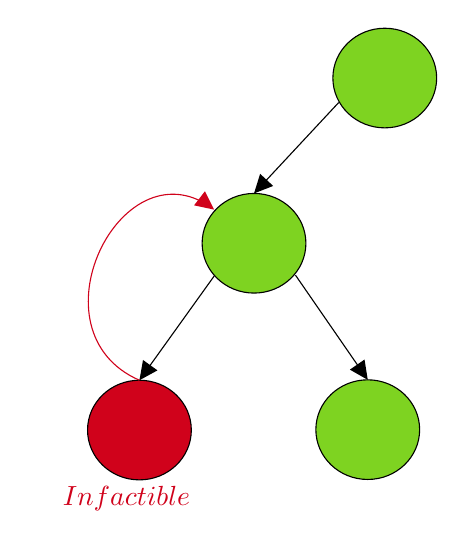
\begin{tikzpicture}[x=0.75pt,y=0.75pt,yscale=-1,xscale=1][h!]
    %uncomment if require: \path (0,300); %set diagram left start at 0, and has height of 300

    %Flowchart: Connector [id:dp4042306815169395] 
    \draw  [fill={rgb, 255:red, 126; green, 211; blue, 33 }  ,fill opacity=1 ] (279,55) .. controls (279,41.75) and (290.19,31) .. (304,31) .. controls (317.81,31) and (329,41.75) .. (329,55) .. controls (329,68.25) and (317.81,79) .. (304,79) .. controls (290.19,79) and (279,68.25) .. (279,55) -- cycle ;
    %Flowchart: Connector [id:dp1116731849912348] 
    \draw  [fill={rgb, 255:red, 126; green, 211; blue, 33 }  ,fill opacity=1 ] (216,134.6) .. controls (216,121.35) and (227.19,110.6) .. (241,110.6) .. controls (254.81,110.6) and (266,121.35) .. (266,134.6) .. controls (266,147.85) and (254.81,158.6) .. (241,158.6) .. controls (227.19,158.6) and (216,147.85) .. (216,134.6) -- cycle ;
    %Flowchart: Connector [id:dp9241040693319311] 
    \draw  [fill={rgb, 255:red, 208; green, 2; blue, 27 }  ,fill opacity=1 ] (160.8,224.6) .. controls (160.8,211.35) and (171.99,200.6) .. (185.8,200.6) .. controls (199.61,200.6) and (210.8,211.35) .. (210.8,224.6) .. controls (210.8,237.85) and (199.61,248.6) .. (185.8,248.6) .. controls (171.99,248.6) and (160.8,237.85) .. (160.8,224.6) -- cycle ;
    %Flowchart: Connector [id:dp8545520848009915] 
    \draw  [fill={rgb, 255:red, 126; green, 211; blue, 33 }  ,fill opacity=1 ] (270.8,224.4) .. controls (270.8,211.15) and (281.99,200.4) .. (295.8,200.4) .. controls (309.61,200.4) and (320.8,211.15) .. (320.8,224.4) .. controls (320.8,237.65) and (309.61,248.4) .. (295.8,248.4) .. controls (281.99,248.4) and (270.8,237.65) .. (270.8,224.4) -- cycle ;
    %Straight Lines [id:da08954787249536511] 
    \draw    (281.8,66.8) -- (243.04,108.4) ;
    \draw [shift={(241,110.6)}, rotate = 312.97] [fill={rgb, 255:red, 0; green, 0; blue, 0 }  ][line width=0.08]  [draw opacity=0] (8.93,-4.29) -- (0,0) -- (8.93,4.29) -- cycle    ;
    %Straight Lines [id:da07941464236907325] 
    \draw    (261,150) -- (294.1,197.93) ;
    \draw [shift={(295.8,200.4)}, rotate = 235.38] [fill={rgb, 255:red, 0; green, 0; blue, 0 }  ][line width=0.08]  [draw opacity=0] (8.93,-4.29) -- (0,0) -- (8.93,4.29) -- cycle    ;
    %Straight Lines [id:da7617271108069388] 
    \draw    (221.8,150.4) -- (187.55,198.16) ;
    \draw [shift={(185.8,200.6)}, rotate = 305.65] [fill={rgb, 255:red, 0; green, 0; blue, 0 }  ][line width=0.08]  [draw opacity=0] (8.93,-4.29) -- (0,0) -- (8.93,4.29) -- cycle    ;
    %Curve Lines [id:da6335093373232185] 
    \draw [color={rgb, 255:red, 208; green, 2; blue, 27 }  ,draw opacity=1 ]   (185.8,200.6) .. controls (132.22,177.16) and (176.43,87.16) .. (219.82,116.95) ;
    \draw [shift={(221.8,118.4)}, rotate = 217.69] [fill={rgb, 255:red, 208; green, 2; blue, 27 }  ,fill opacity=1 ][line width=0.08]  [draw opacity=0] (8.93,-4.29) -- (0,0) -- (8.93,4.29) -- cycle    ;
    % Text Node
    \draw (147.6,250.6) node [anchor=north west][inner sep=0.75pt]  [color={rgb, 255:red, 208; green, 2; blue, 27 }  ,opacity=1 ]  {$Infactible$};

    \end{tikzpicture}
\end{center}





